\begin{frame}[fragile]{\insertsubsection}

  \begin{onlyenv}<1>
    \begin{minted}[fontsize = \footnotesize, gobble = 4, frame = lines, framesep
      = 7pt, label = Rust, linenos, breaklines]{rust}
    impl<'a, 'gcx, 'tcx> InferCtxt<'a, 'gcx, 'tcx> {
        pub fn replace_bound_vars_with_placeholders<T>(&self,
          binder: &ty::Binder<T>) -> (T, PlaceholderMap<'tcx>)
        where T: TypeFoldable<'tcx>
        {
            let next_universe = self.create_next_universe();
            let fld_r = |br| {
                self.tcx.mk_region(ty::RePlaceholder(ty::PlaceholderRegion {
                    universe: next_universe,
                    name: br,
                }))
            };
            ...
        }
    }
      \end{minted}
  \end{onlyenv}

  \begin{onlyenv}<2>
    \center%
    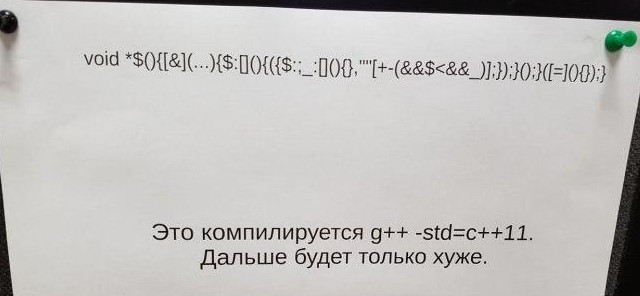
\includegraphics[width = \textwidth]{c_p_p_syntax.jpg}
  \end{onlyenv}

  \note<1>{

    Незнакомых с Rust очень сильно \textbf{отпугивает сложный синтаксис} ---
    зачем все эти закорючки, зачем сокращать слова, зачем столько скобок и т. д.
    Суть в том, что это \textbf{язык без GC}, со своей, \textbf{особой техникой
      отслеживания времени жизни объекта}, отсюда такой комплексный синтаксис, к
    которому привыкаешь. Если хотите писать на безопасном и быстром языке, от
    этого никуда не деться.

    \textbf{Лично по моему опыту} --- когда я начинал изучать Rust, он не был
    таким популярным, в итоге на форумах никто не брюзжал о том, что синтаксис
    плох. И когда я изучал Rust у меня не было практически никакого мнения о
    нём, я знал, для чего он и что может, но как он изучается --- в курсе не
    был. В итоге синтаксис мне не показался чем-то сложным, бо́льшие сложности у
    меня возникли \textbf{при осознании построения правильных и идиоматичных
      абстракций} в Rust. Стоит заметить, что \textbf{раньше синтаксис был ещё
      комплекснее}, это сейчас делают всё, чтобы компилятор понимал, чего хочет
    программист.

    Прелесть Rust в том, что в нём сложный процесс написания кода. То есть вы
    часть ошибок ловите ещё до этапа компиляции. То есть вы вынуждены больше
    думать наперёд, и в итоге получаете меньше проблем.

  }

  \note<2>{

    И вообще, многое \textbf{зависит от самого разработчика}, как он сам напишет
    код, потому что уродливо можно написать на любом языке, каким бы лаконичным
    он ни был.

    \textbf{Лично мне синтаксис Rust никогда не казался сложным или непонятным},
    даже наоборот, \textbf{я нахожу его более понятным}.

    \begin{itemize}
    \item Чётко видно где и какие методы используются, где они реализованы (а не
      \textbf{блуждать в include файлах}).
    \item Чётко понимаю, какой тип у переменной.
    \item Понимаю какой знак к чему относится (C pointers).
    \item Код легче читать, потому что всё обернуто в абстракции типов.
    \item Ясно что и куда передаётся в разных потоках.
    \end{itemize}

  }
\end{frame}
